\subsubsection{Implementation on STM32}
In a first iteration of the implementation and subsequent testing, the STM32 was used, by implementing the control algorithm in equation~\ref{equ:pid-discrete-veloc-modif} in a program designed to create command variables through simulated measurements of the desired control variables, the command variables would then act upon the simulated system model in equation~\ref{equ:sysModel} that would then return the measured variables for the controller to use; thus the real system's controller and behaviour can be simulated.
The command variables and control variables are placed on a buffer for each iteration and at the end of the simulation the values are sent to an interface for analysis.
\subsubsection{STM32 Program}

The program utilizes two timer triggered ISRs with the same period, that of fifty miliseconds. However the system response ISR where the command variables shall act upon the system is offset by 500 ticks thus ensuring that the ISRs shall never be triggered at the same time whilst still having the same period. \\
Starting with the system ISR (Fig.~\ref{fig:kinModeCode}), firstly obtaining the psi required for the model, which is done integrating psidot, which, in discrete time, is done through the summation of the product of the current psidot and the sampling time added to the summation of all previous psidot multiplied by the sampling time (this latter summation is called aux\textunderscore psi). Then measuring the velocity and, with this information, calculate the next x and y components of the linear velocity of the rover. After that integrate nVx and nVy the same way psi was, and obtaining the position of the car on the x and y axis; followed by obtaining Vr\textunderscore m and Vl\textunderscore m through the norm.
\begin{figure}[!htbp]
\centering
       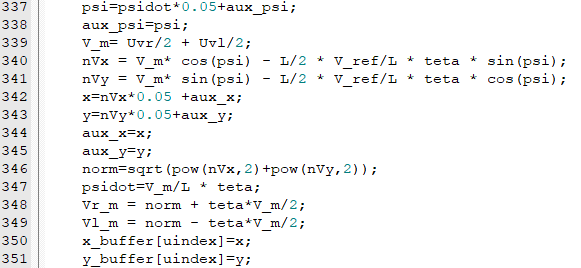
\includegraphics[page=1,width=0.6\textwidth]{img/sysCode.png} 
\caption{System model converted into lines of code}
\label{fig:kinModeCode}
\end{figure}
\\
Next is the implementation of the controller. Firstly the obstacle avoidance (Fig.~\ref{fig:odomCode}), it is done through a sensor\textunderscore buffer, which, whenever one of the nine sensors (with a field angle of $\frac{2\pi}{9}$ rads) detects a nearby obstacle, a one will be placed on the index it is related to (the sensor that detects from 0 rad to  $\frac{2\pi}{9}$ rad is related to index one then from $\frac{2\pi}{9}$ rad to $\frac{4\pi}{9}$ rad is index two and so on until $2\pi$ rad) from that buffer the controller interprets the angles which are not permitted, this is done thorough a "for" cycle that searches for ones on the buffer and through the corresponding index calculates the boundaries of the unpermitted angles; should the currently desired variation of steering angle (psidot) lead towards anywhere within the boundaries of those angles, the reference variables are set to zero and the controller will stop the car.
\begin{figure}[!htbp]
\centering
       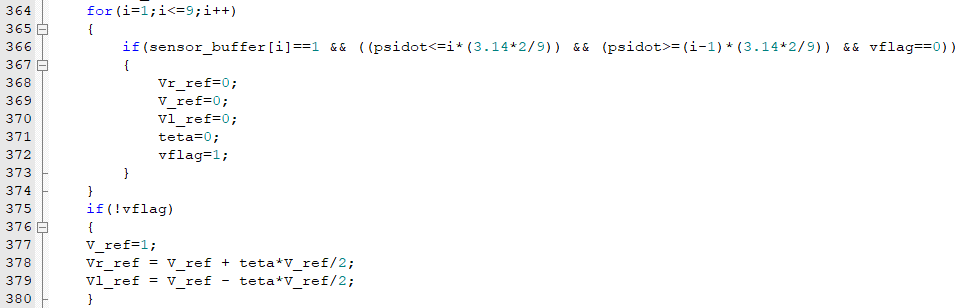
\includegraphics[page=1,width=0.8\textwidth]{img/odometryCode.png} 
\caption{Obstacle avoidance algorithm}
\label{fig:odomCode}
\end{figure}
\\
The controller (Fig.~\ref{fig:controllerCode}) follows the equation~\ref{equ:pid-discrete-veloc-modif}, as previously stated, therefore it was merely converted without a kd; for the optimal control obtained in previous chapters was with kd=0.
\begin{figure}[!htbp]
\centering
       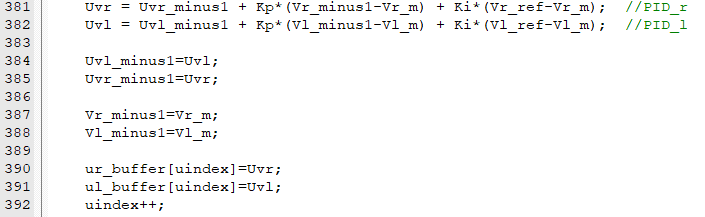
\includegraphics[page=1,width=0.8\textwidth]{img/controllerCode.png} 
\caption{Controller converted into lines of code}
\label{fig:controllerCode}
\end{figure}